\documentclass[12pt,a4paper,austrian]{article}
\usepackage{graphicx}
\usepackage[austrian, english]{babel}
\usepackage[utf8]{inputenc}
%\usepackage{listings}
\usepackage{multirow}
\usepackage{epstopdf}
\usepackage{amsmath}
\usepackage{amssymb} % fuer Mengen \N, Q, C, R
\graphicspath{{./fig/}}


%% Satzspiegel
\setlength{\hoffset}{-1in} \setlength{\textwidth}{18cm}
\setlength{\oddsidemargin}{1.5cm}
\setlength{\evensidemargin}{1.5cm}
\setlength{\marginparsep}{0.7em}
\setlength{\marginparwidth}{0.5cm}

\setlength{\voffset}{-1.9in}
\setlength{\headheight}{12pt}
\setlength{\topmargin}{2.6cm}
   \addtolength{\topmargin}{-\headheight}
\setlength{\headsep}{3.5cm}
   \addtolength{\headsep}{-\topmargin}
   \addtolength{\headsep}{-\headheight}
\setlength{\textheight}{27cm}

%% How should floats be treated?
\setlength{\floatsep}{12 pt plus 0 pt minus 8 pt}
\setlength{\textfloatsep}{12 pt plus 0pt minus 8 pt}
\setlength{\intextsep}{12 pt plus 0pt minus 8 pt}

\tolerance2000
\emergencystretch20pt

%% Text appearence
% English text
\newcommand{\eg}[1]%
  {\selectlanguage{english}\textit{#1}\selectlanguage{austrian}}

\newcommand{\filename}[1]
  {\begin{small}\texttt{#1}\end{small}}

\newcommand\IFT{\unitlength1mm\begin{picture}(10,2) \put (1,1)
{\circle{1.7}} \put(2,1){\line(1,0){5}} \put(8,1)
{\circle*{1.7}}\end{picture}}
\newcommand\FT{\unitlength1mm\begin{picture}(10,2) \put (1,1)
{\circle*{1.7}} \put(2,1){\line(1,0){5}} \put(8,1)
{\circle{1.7}}\end{picture}}

% A box for multiple choice problems
\newcommand{\choicebox}{\fbox{\rule{0pt}{0.5ex}\rule{0.5ex}{0pt}}}

\newenvironment{wahrfalsch}%
  {\bigskip\par\noindent\makebox[1cm][c]{richtig}\hspace{3mm}\makebox[1cm][c]{falsch}
   \begin{list}%
   {\makebox[1cm][c]{\choicebox}\hspace{3mm}\makebox[1cm][c]{\choicebox}}%
   {\setlength{\labelwidth}{2.31 cm}\setlength{\labelsep}{3mm}
    \setlength{\leftmargin}{2.61 cm}\setlength{\listparindent}{0pt}
    \setlength{\itemindent}{0pt}}%
  }
  {\end{list}}

\newcounter{theaufgabe}\setcounter{theaufgabe}{1}
\newenvironment{aufgabe}[1]%
  {\bigskip\par\noindent\begin{nopagebreak}
   \textsf{\textbf{\arabic{theaufgabe}.\thinspace Aufgabe}}\quad
      \textsf{\textit{#1}}\\*[1ex]%
\stepcounter{theaufgabe}\hspace{2ex}\end{nopagebreak}}
  {\par\pagebreak[2]}

% Innerhalb der Aufgaben erfolgt die weitere Unterteilung mittels einer
% enumerate Umgebung, die allerdings a), b),... zaehlen soll.
\renewcommand{\labelenumi}{\alph{enumi})}
\renewcommand{\labelenumii}{\arabic{enumii})}

% A box to tick for everything which has to done
\newcommand{\abgabe}{\marginpar{$\Box$}}
% Margin paragraphs on the left side
\reversemarginpar

% Language for listings
%\lstset{language=Vhdl,
%  basicstyle=\small\tt,
 % keywordstyle=\tt\bf,
 % commentstyle=\sl}

% No indention
\setlength{\parindent}{0.0cm}
% Don't number sections
\setcounter{secnumdepth}{0}


%% Beginning of the text

\begin{document}
\selectlanguage{austrian}
\pagestyle{plain}


%===  This is the header section ============================================================
\thispagestyle{empty}
\noindent
\begin{minipage}[b][4cm]{1.0\textwidth}  
\begin{center}
\begin{bf} 
\begin{large} Digital Signal Processing SS 2024 -- 1.~Assignment\end{large} \\
\vspace{0.3cm}
\begin{Large} Analogue Signals and Systems  \end{Large} \\
\vspace{0.3cm}
\end{bf}
\begin{large}
Group 22\\
Julian Feichtinger, K12015812\\
Wolfram Laube, K08900915\\
\end{large} 
\end{center}
\end{minipage}

\noindent \rule[0.8em]{\textwidth}{0.12mm}\\[-0.5em]
%=======================================================================================


\begin{aufgabe}{Discrete Time Signals (30\%)}

The following discrete time signals should be plotted in Matlab as indicated in Figure 1.
\[
\begin{array}{ll}
x_{1}[n] = -4 \delta[n+3] + 4 \delta[n] - \delta[n-3] + 2 \delta[n-7] & \text{for } -5 \leq n \leq 10 \\
x_{2}[n] = e^{-0.31 n} & \text{for } -5 \leq n \leq 10 \\
x_{3}[n] = 3 \sin \left(2 \pi \frac{3.5}{64} n\right) & \text{for } 0 \leq n \leq 256 \\
x_{4}[n] = -\cos \left(\frac{9}{64} n\right) & \text{for } 0 \leq n \leq 256
\end{array}
\]
To indicate the discrete time nature of the signals, the \texttt{stem} command should be used, unless the signal length becomes too long, in which case the \texttt{plot} command should be used instead. Choose the ideal way to plot the signals.
Extend the Matlab script \texttt{dsp\_A2\_1.m}. Useful commands are \texttt{figure}, \texttt{stem}, \texttt{plot}, \texttt{subplot}, \texttt{xlabel}, \texttt{ylabel}, \texttt{title}, \texttt{legend}, \texttt{hold on}, \texttt{grid on}, \texttt{pi}.
You can use the provided function \texttt{impseq}.

\begin{figure}[h]
\centering
\includegraphics[width=\textwidth]{fig/ex2_fourier_transformed}
\caption{Required arrangement of plots}
\end{figure}

\subsection*{(b) Normalized Angular Frequency $\Omega$}
What is the normalized angular frequency $\Omega$ for $x_{3}[n]$ and $x_{4}[n]$?

\subsection*{(c) Periodicity of Signals}
Are the signals $x_{3}[n]$ and $x_{4}[n]$ periodic? If yes, what is their fundamental period?

\subsection*{(d) Matlab Function \texttt{custom\_power}}
Write the Matlab function \texttt{custom\_power} which calculates the mean power of a discrete time periodic signal according to
\[ P = \frac{1}{N} \sum_{n=0}^{N-1} |x[n]|^2 \]
Pass exactly one signal period to this function to calculate the powers of all periodic signals in (a).

\subsection*{(e) Function \texttt{energy} and Signal Energies}
Now assume that all signals in (a) are zero outside the plot range (e.g., $x_{2}[11] = 0$).

Write a function \texttt{energy} which calculates the signal energy according to
\[ W = \sum_{n=-\infty}^\infty |x[n]|^2 \]
Determine the energies for all these time-limited signals $x_{1}[n]$ to $x_{4}[n]$.

\subsection*{(f) Table of Signal Powers and Energies}
Collect all the signal powers of (d) and signal energies of (e) in a single table in your protocol.


\hrule

%%! Author = wolfram_e_laube
%! Date = 02.04.24

\textbf{Form Conversions}

\begin{enumerate}
\item[-]
$c_2 = \frac{\sqrt{2}}{2} e^{-\frac{j 3 \pi}{4}}$ to rectangular form:
\[
\begin{aligned}
& x = \frac{\sqrt{2}}{2} \cos({-\frac{3 \pi}{4}}) = \frac{\sqrt{2}}{2} \cdot -\frac{\sqrt{2}}{2} = -\frac{1}{2} \\
& y = \frac{\sqrt{2}}{2} \sin({-\frac{3 \pi}{4}}) = \frac{\sqrt{2}}{2} \cdot -\frac{\sqrt{2}}{2} = -\frac{1}{2} \\
& c_2 = -\frac{1}{2} - j \frac{1}{2}
\end{aligned}
\]
\end{enumerate}

\textbf{Calculations}

\begin{enumerate}
\item[-]
$c_4 = c_1 + c_2$: To add, we use $c_2$ in rectangular form as calculated above:
\[
\begin{aligned}
& c_4 = (-5 - \frac{1}{2}) + (3 - \frac{1}{2})j = -\frac{11}{2} + j \frac{5}{2}
\end{aligned}
\]
\end{enumerate}

\begin{enumerate}
\item[-]
$c_5 = c_1 \cdot c_2$: For multiplication, too:
\[
\begin{aligned}
& c_5 = c_1 \cdot c_2 = (-5+j 3) \cdot (-\frac{1}{2} - j \frac{1}{2}) = \\
& = (-5)\cdot (- \frac{1}{2})  + j(-5)\cdot(-\frac{1}{2}) + j3\cdot(-\frac{1}{2})+ j^23\cdot(-\frac{1}{2}) = \\
& = \frac{5}{2}+\frac{3}{2} +j(\frac{5}{2}-\frac{3}{2}) = 4 + j
\end{aligned}
\]
\end{enumerate}

\begin{enumerate}
\item[-]
$c_6 = |c_3|^2$: Square each component of $c_3$ and sum up:
\[
\begin{aligned}
& c_6 = \frac{1}{\sqrt{2}}^2 + \frac{1}{\sqrt{2}}^2 = 1
\end{aligned}
\]
\end{enumerate}

\begin{enumerate}
\item[-]
$c_7 = \arg(c_3)$: is in the first quadrant (both real and imaginary parts positive):
\[
\begin{aligned}
& c_7 = \arg(c_3) = \arctan\left(\frac{1}{\sqrt{2}}/\frac{1}{\sqrt{2}}\right) = \arctan(1) = \pi/4
\end{aligned}
\]
\end{enumerate}

\begin{enumerate}
\item[-]
$c_8 = \frac{c_1}{c_2}$: Expand with conjugate complex of denominator:
\[
\begin{aligned}
& c_8 = \frac{c_1\cdot c_2^*}{c_2 \cdot c_2^*} = \\
& = \frac{1}{|c_2^*|^2} \cdot (c_1 \cdot c_2^*) = \\
& = 2 \cdot ((-5+j 3)) \cdot (-\frac{1}{2} + j \frac{1}{2}) = \\
& = 2 \cdot (1 - j4) = 2 - j8
\end{aligned}
\]
\end{enumerate}

\begin{enumerate}
\item[-]
$c_9 = c_1 * c_1^*$: Multiply directly or use $c_1 \cdot c_1^* = |c_1|^2$:
\[
\begin{aligned}
& c_1^* = -5 - 3j \\
& c_9 = (-5 + 3j) \cdot (-5 - 3j) = 25 + j15 -j15 -j^29 = 34
\end{aligned}
\]
\end{enumerate}


\end{aufgabe}

\begin{aufgabe}{Fourier Transform (25\%)}

The signal $x[n]=(3,-1,2,0,1)$ at sample times $n=(0,1,2,3,4)$ is the input to an LTI system with impulse response $h[n]=(2,3,4,1)$ at sample times $n=(0,1,2,3)$.

\subsection{(a) Output Signal Length}
How long is the output signal $y[n]$?

\subsection{(b) Manual Calculation of $y[n]$}
Manually calculate the output signal $y[n]$.

\hrule

\begin{enumerate}
%%! Author = wolfram_e_laube
%! Date = 02.04.24

\item [a)]
Given the cosine wave expressed as
$$
x(t) = \hat{X} \cos(2\pi f_0 t),
$$
we aim to prove its Fourier transform pair. Using Euler's formula, $\cos(\theta) = \frac{e^{j\theta} + e^{-j\theta}}{2}$, we can express the cosine function as a sum of complex exponentials:
$$
x(t) = \hat{X} \left( \frac{e^{j2\pi f_0 t} + e^{-j2\pi f_0 t}}{2} \right) = \frac{\hat{X}}{2} e^{j2\pi f_0 t} + \frac{\hat{X}}{2} e^{-j2\pi f_0 t}.
$$

The Fourier transform of a complex exponential function is given by:
$$
e^{j2\pi f_0 t} \leftrightarrow \delta(f-f_0)
$$
and
$$
e^{-j2\pi f_0 t} \leftrightarrow \delta(f+f_0).
$$

Therefore, applying the Fourier transform to $x(t)$, we obtain:
$$
X(f) = \frac{\hat{X}}{2} \delta(f-f_0) + \frac{\hat{X}}{2} \delta(f+f_0),
$$
proving the given Fourier transform pair for the cosine wave.


%%! Author = wolfram_e_laube
%! Date = 02.04.24

\item [b)]
Figure~\ref{fig:FourierTransform} shows the Fourier transformed of the above function. \\
\begin{figure}[!ht]
	\centering
	\includegraphics[width=18cm]{ex2_fourier_transformed.eps}
	\vspace{-0.3cm}
	\caption{Fourier Transform.}
	\label{fig:FourierTransform}
	\vspace{-0.1cm}
\end{figure}

\end{enumerate}

\end{aufgabe}

\begin{aufgabe}{Time Shift and Phase (20\%)}
Given are two sines according to the following formula with $f_{1}=1 \mathrm{~Hz}$ and $f_{2}=3 \mathrm{~Hz}$.

$$
x_{i}(t)=\sin \left(2 \pi f_{i} t\right), \text { with } i \in\{1,2\}
$$

All two sines are time delayed by $\tau=0.1 \mathrm{~s}$ to yield

$$
y_{i}(t)=\sin \left(2 \pi f_{i}(t-0.1)\right) \text {. }
$$

This corresponds to a phase shift. Thus, the delayed sines may also be written as

$$
y_{i}(t)=\sin \left(2 \pi f_{i} t+\phi_{i}\right) .
$$

\begin{enumerate}
\item[a)] Calculate the phase shifts $\phi_{i}$ for each sine, and verify that this corresponds to the 'Shift Theorem' of the
Fourier Transform (DSP\_2.pdf, page 41).

\item[b)] For both sines in separated plots: Plot the original signal, the time delayed signal and the phase shifted signal.
Since the latter two are identical, show this by plotting the first with a solid line and the overlaid one in a
different colour with a dashed line. Plot each signal from 0 to $1 \mathrm{~s}$.
In Matlab use the following time-vector: $\mathrm{t}=0: 0.001: 1$.
\end{enumerate}

\hrule

\begin{enumerate}
%\item[(a)]
\section*{Exercise 3 Task (a): Frequency Analysis of \(x(t)\)}

\subsection*{Objective}
This task involves identifying all positive frequencies up to 20 kHz in the analog signal \(x(t)\), derived from the discrete-time signal \(x[n]\) through a DAC operating at 8 kHz.

\subsection*{Methodology}
The discrete-time signal \(x[n] = \sqrt{2} \cdot \sin\left(2\pi \frac{1}{8} n\right)\) has a fundamental frequency \(f_0 = 1 \text{kHz}\) because it completes \(\frac{1}{8}\) of a cycle per sample, and the DAC operates at 8 kHz. The analysis focuses on the effects of sampling, which replicates the spectrum around multiples of the sampling frequency, leading to potential frequencies at:
\(f_0\),
\(f_s \pm f_0\),
\(2f_s \pm f_0\)
etc., where \(f_s\) is the sampling frequency (8 kHz).

\subsection*{Results}
The positive frequencies identified in \(x(t)\) and shown in Figure~\ref{fig:exercise3a_frequencies} are:
\begin{itemize}
\item 1 kHz (base frequency)
\item 7 kHz (\(8 \text{ kHz} - 1 \text{ kHz}\))
\item 9 kHz (\(8 \text{ kHz} + 1 \text{ kHz}\))
\item 15 kHz (\(16 \text{ kHz} - 1 \text{ kHz}\))
\item 17 kHz (\(16 \text{ kHz} + 1 \text{ kHz}\))
\end{itemize}

\begin{figure}[h]
    \centering
    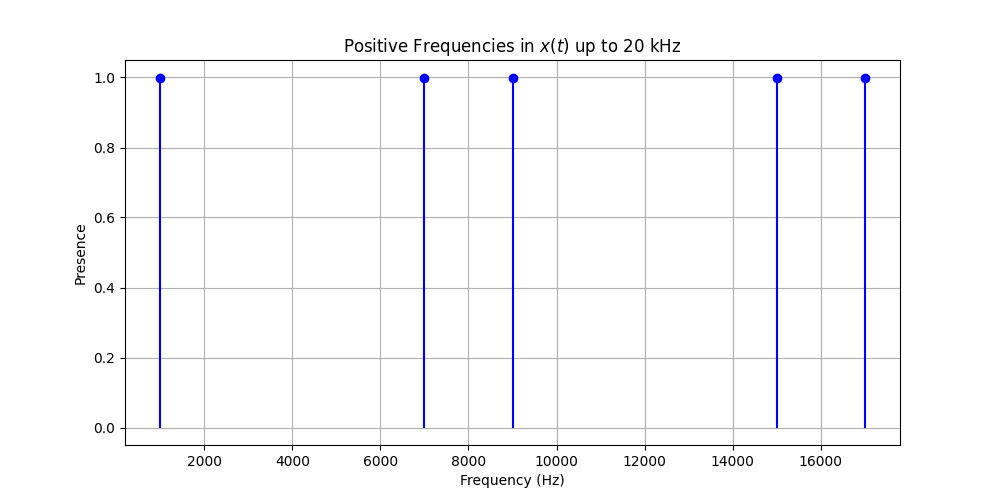
\includegraphics[width=0.8\textwidth]{fig/ex3_task_a_frequencies}
    \caption{Positive frequencies in \(x(t)\) up to 20 kHz}
    \label{fig:exercise3a_frequencies}
\end{figure}

\subsection*{Conclusion}
This detailed frequency analysis underscores the significance of understanding the effects of sampling on the signal's spectrum.
It aids in designing digital systems that effectively manage aliasing and maintain signal fidelity.

%%! Author = wolfram_e_laube
%! Date = 02.04.24

\item [b)]
Plotting the Signals

Figure~\ref{fig:SignalPlot} shows two subplots, one for each frequency. In each subplot, it plots the original signal,
the time-delayed signal (in red dashed lines), and the phase-shifted signal (in green dot-dashed lines,
slightly transparent for better visibility).
The time-delayed and phase-shifted signals are expected to overlap completely,
demonstrating that a time delay is equivalent to a phase shift in the time domain.
\begin{figure}[!ht]
	\centering
	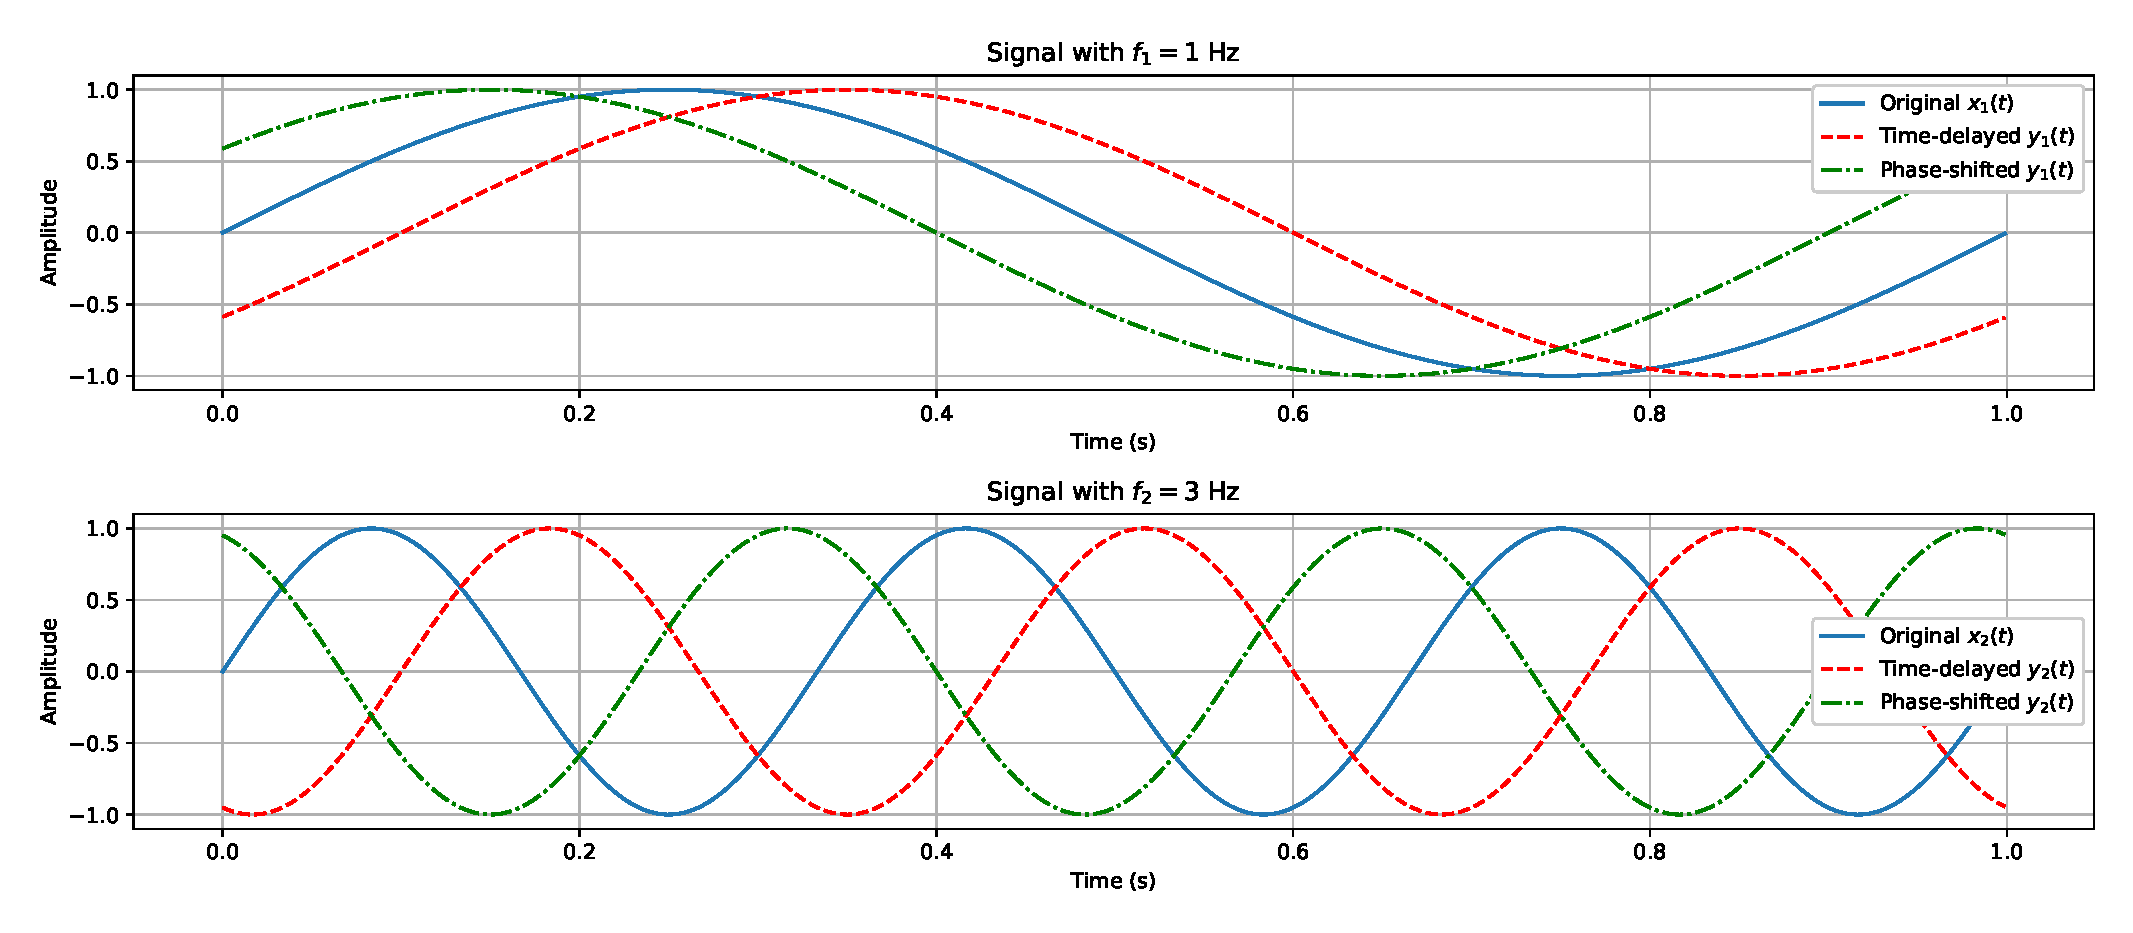
\includegraphics[width=18cm]{ex3_signal_plot.eps}
	\vspace{-0.3cm}
	\caption{Signal Plot.}
	\label{fig:SignalPlot}
	\vspace{-0.1cm}
\end{figure}



\end{enumerate}

\end{aufgabe}

\begin{aufgabe}{Linearity and Time Invariance (35\%)}
Examine the following systems (input $x(t)$ and output $y(t)$ ) for linearity and time invariance.

Clearly show the mathematical derivations and state if the systems are linear and/or time-invariant.

\begin{enumerate}
\item[a)] $y(t)=(x(t))^{2}$
\item[b)] $y(t)=x(t) \cdot \sin \left(\Omega_{0} t\right)$
\end{enumerate}

\hrule

\begin{enumerate}
%%! Author = wolfram_e_laube
%! Date = 02.04.24

\item[a)]
System 1: $y(t)=x(t)^{2}$

\textbf{Linearity Test:}

To test for linearity, consider two inputs, $x_1(t)$ and $x_2(t)$, and constants $a$ and $b$. The system's response to the combination $a x_1(t) + b x_2(t)$ is:

$$
y(t) = \left(a x_1(t) + b x_2(t)\right)^2
$$

Expanding this expression gives:

$$
y(t) = a^2 (x_1(t))^2 + 2ab x_1(t) x_2(t) + b^2 (x_2(t))^2
$$

This result does not equal $a (x_1(t))^2 + b (x_2(t))^2$ (which would be $a y_1(t) + b y_2(t)$), indicating that the system does not satisfy the linearity property.

\textbf{Time Invariance Test:}

Consider an input $x(t - \tau)$ which produces the output:

$$
y(t) = (x(t - \tau))^2
$$

This output directly corresponds to squaring the time-shifted input, which means the system is time-invariant.

\textbf{Conclusion for System 1:} The system is not linear but is time-invariant.
%%! Author = wolfram_e_laube
%! Date = 02.04.24

\item[b)]
System 2: $y(t)=x(t) \cdot \sin \left(\Omega_{0} t\right)$

\textbf{Linearity Test:}

For inputs $x_1(t)$ and $x_2(t)$, and constants $a$ and $b$, the system's response to the combination
$a x_1(t) + b x_2(t)$ is:

$$
y(t) = (a x_1(t) + b x_2(t)) \cdot \sin(\Omega_0 t)
$$

This simplifies to:

$$
y(t) = a x_1(t) \sin(\Omega_0 t) + b x_2(t) \sin(\Omega_0 t)
$$

This result is equal to $a y_1(t) + b y_2(t)$, indicating that the system satisfies the linearity property.

\textbf{Time Invariance Test:}

Consider an input $x(t - \tau)$ which produces the output:

$$
y(t) = x(t - \tau) \cdot \sin(\Omega_0 t)
$$

This output is not equivalent to $y(t - \tau) = x(t - \tau) \cdot \sin(\Omega_0 (t - \tau))$,
indicating that the system does not satisfy the time invariance property because the sine function's phase
is affected by the time shift.

\textbf{Conclusion for System 2:} The system is linear but not time-invariant.

\end{enumerate}

\end{aufgabe}


\end{document}
